%{{{ Formatierung

\documentclass[a4paper,12pt]{article}

\usepackage{physics_notetaking}

%%% dark red
%\definecolor{bg}{RGB}{60,47,47}
%\definecolor{fg}{RGB}{255,244,230}
%%% space grey
%\definecolor{bg}{RGB}{46,52,64}
%\definecolor{fg}{RGB}{216,222,233}
%%% purple
%\definecolor{bg}{RGB}{69,0,128}
%\definecolor{fg}{RGB}{237,237,222}
%\pagecolor{bg}
%\color{fg}

\newcommand{\td}{\,\text{d}}
\newcommand{\RN}[1]{\uppercase\expandafter{\romannumeral#1}}
\newcommand{\zz}{\mathrm{Z\kern-.3em\raise-0.5ex\hbox{Z} }}

\newcommand\inlineeqno{\stepcounter{equation}\ {(\theequation)}}
\newcommand\inlineeqnoa{(\theequation.\text{a})}
\newcommand\inlineeqnob{(\theequation.\text{b})}
\newcommand\inlineeqnoc{(\theequation.\text{c})}

\newcommand\inlineeqnowo{\stepcounter{equation}\ {(\theequation)}}
\newcommand\inlineeqnowoa{\theequation.\text{a}}
\newcommand\inlineeqnowob{\theequation.\text{b}}
\newcommand\inlineeqnowoc{\theequation.\text{c}}

\renewcommand{\refname}{Source}
\renewcommand{\sfdefault}{phv}
%\renewcommand*\contentsname{Contents}

\pagestyle{fancy}

\sloppy

\numberwithin{equation}{section}

%}}}

\begin{document}

%{{{ Titelseite

\title{physik311 $|$ Notizen}
\author{Jonas Wortmann}
\maketitle
\pagenumbering{gobble}

%}}}

\newpage

%{{{ Inhaltsverzeichnis

\fancyhead[L]{\thepage}
\fancyfoot[C]{}
\pagenumbering{arabic}

\tableofcontents

%}}}

\newpage

%{{{

\fancyhead[R]{\leftmark\\\rightmark}

\section{Einführung}
Licht ist eine elektromagnetische Welle. Die Wellenlänge ist im Bereich von $\SI{400}{nm}$ bis $\SI{800}{nm}$, das entspricht einer Frequenz von $\SI{750}{THz}$ bis $\SI{375}{THz}$. Ein Lichtpuls kann nie kürzer als ein Zyklus sein.

\subsection{Lichtquellen}
\begin{enumerate}[label=--]
        \item Lampe: Inkoherentes (\glqq ungeordnetes\grqq{}) Licht
        \item Laser: Koherentes (\glqq geordnetes\grqq{}, auch Wellen in \glqq gleichschritt\grqq{}) Licht
\end{enumerate}

\newpage
\section{Die elektromagnetische Theorie des Lichts}
Für diesen Fall betrachtet man nur die Lichtausbreitung in großer Entfernung von allen Quellen. Also ist $\rho =0$ und $\vv{j}=0$. Die \textsc{Maxwell}--Gleichungen sind dann
\begin{align}
        \,\text{div}\,\vv{D}&=0\\
        \,\text{div}\,\vv{B}&=0\\
        \,\text{rot}\,\vv{E}&=-\diffp[]{\vv{B}}{t}\\
        \,\text{rot}\,\vv{H}&=\diffp[]{\vv{D}}{t}
.\end{align}
In Materialien gilt dann
\begin{align} 
        \vv{D}&=\varepsilon \varepsilon _0\vv{E}\\
        \vv{B}&=\mu \mu _0\vv{H}
.\end{align} 
Hier ist $\varepsilon $ die Dielektrizitätskonstante und $\mu $ die relative Permeabilität (in der Optik ist sie üblicherweise 1). \\\indent
\begin{align} 
        \,\text{rot}\,\left(\,\text{rot}\,\vv{E}\right)&=\underbrace{\,\text{div}\,\left(\,\text{div}\,\vv{E}\right)}_{=0}-\,\text{div}\,\,\text{grad}\,\vv{E}\\
                                                       &=\,\text{rot}\,\left(-\diffp[]{\vv{B}}{t}\right)
.\end{align} 
Mit $\,\text{rot}\,\vv{B}=\varepsilon\mu \varepsilon _0 \mu _0\diffp[]{\vv{E}}{t}$ folgt
\begin{align} 
        \,\text{div}\,\,\text{grad}\,\vv{E}&=\varepsilon \mu \varepsilon _0\mu _0\diffp[2]{\vv{E}}{t}
.\end{align} 
Dies ist die \textbf{Wellengleichung} für das elektrische Feld. Man erwartet eine Ausbreitungsgeschwindigkeit mit
\begin{align} 
        v_{\,\text{ph}\,}&=\dfrac{1}{\,\sqrt[]{\varepsilon \mu \varepsilon _0\mu _0}}\equiv \dfrac{c}{n}
,\end{align} 
wobei $c=\,\sqrt[]{\varepsilon _0\mu _0}^{-1}$ die Vakuumslichtgeschwindigkeit und $n=\,\sqrt[]{\varepsilon \mu }$ der Brechungsindex ist. Dann lässt sich die Wellengleichung wie folgt schreiben
\begin{align} 
        \,\text{div}\,\,\text{grad}\,\vv{E}&=\dfrac{1}{v_{\,\text{ph}\,}^2}\diffp[2]{\vv{E}}{t}\stackrel{\,\text{Vakuum}\,}{=}\dfrac{1}{c^2}\diffp[2]{\vv{E}}{t}
.\end{align} 
Eine analoge Rechnung kann auch für das $\vv{B}$--Feld verwendet werden.\\\indent

\subsection{Einfachste Lösung der Wellengleichung: Ebene elektromag.\ Welle}
Hier wird die Lichtausbreitung nur entlang einer Koordinate (z.B.\ $z$) betrachtet. Also ist $\vv{E}\left(\vv{r},t\right)=\vv{E}\left(z,t\right)$, bzw.\ $\diffp[]{\vv{E}}{x}=\diffp[]{\vv{E}}{y}=0$. Die Wellengleichung vereinfacht sich dann zu
\begin{align} 
        \diffp[2]{\vv{E}}{z}=\dfrac{1}{c^2}\diffp[2]{\vv{E}}{t}
.\end{align} 
Mit $\,\text{div}\,\vv{E}=0$ folgt für ebene Wellen $\diffp[]{E}{z}=0$, also ist $E_z=\,\text{const.}\,$.\\\indent
Jetzt wählt man die Randbedingungen, dass $E_z=0$. Also ist $\vv{E}=\begin{pmatrix}
        E_x\left(z\right)\\E_y\left(z\right)\\0
\end{pmatrix}$. Die Lösung der Wellengleichung ist dann
\begin{align} 
        \vv{E}\left(z,t\right)&=\vv{E}_0\cos \left(kz-\omega t\right)\\
                              &=\vv{E}_0\cos \left(k\left(z-ct\right)\right)
,\end{align} 
wobei $\tfrac{\omega }{k}=c$, mit $k=\tfrac{2\pi }{\lambda }$ der \textbf{Wellenzahl} ($\lambda $ der Wellenlänge) und $\vv{E}_0$ der Amplitude.\\\indent
Die Transversalität (also die Ausbreitung nach oben und unten, $\vv{E}\perp \vv{e}_z$, allg.\ $\vv{E}_z\perp \vv{k}$) folgt aus $\,\text{div}\,\vv{E}=0$ im ladungsfreien Raum. In Medien mit Raumladungen oder an Oberflächen ist auch eine longitudinale Polarisation möglich. Bisher gab es nur lineare Polarisationen; es ist aber auch eine Überlagerung von $E_x$ und $E_y$ möglich. Diese sind zirkulare und elliptische Polarisation.\\\indent
Die Allgemeine Wellengleichung ist
\begin{align} 
        \,\text{div}\,\,\text{grad}\,\vv{E}=\left(\dfrac{n}{c}\right)^2\diffp[2]{\vv{E}}{t}
,\end{align} 
mit $v_{ph}=\tfrac{c}{n}$. Man erlaubt nun die Ausbreitung in eine beliebige Richtung sowie eine allgemeine Phase $\varphi $. Die Lösung ist dann
\begin{align} 
        \vv{E}\left(\vv{r},t\right)=\vv{E}_0\cos \left(\vv{k}\vv{r}-\omega t+\varphi \right)
.\end{align} 
Diese Gleichung erfüllt die Wellengleichung, wenn
\begin{align} 
        \vv{k}^2=\dfrac{n^2\omega ^2}{c^2}
.\end{align} 
Man bezeichnet sie auch als \textbf{Dispersionsrelation}.\\\indent
Aus den \textsc{Maxwell}--Gleichungen ist bekannt, dass
\begin{align} 
        \vv{B}=\dfrac{1}{\omega }\left(\vv{k}\times \vv{E}\right)
.\end{align} 
Das zeigt, dass $\vv{B}\perp \vv{E}\land \vv{k}$ und $|\vv{B}|=\tfrac{n}{c}|\vv{E}|$.\\\indent
Die Ursache der Wechselwirkung zwischen Licht und Materie ist überwiegend der elektrische Anteil der Welle (im sichtbaren Bereich).\\\indent
$\vv{E}$ und $\vv{B}$ sind nur im Fernfeld in Phase.

\subsection{Energie und Impuls von Licht}
Zuerst wird die Energiedichte des elektromagnetischen Feldes im Vakuum eingeführt
\begin{align} 
        W_{\,\text{el}\,}&=\dfrac{1}{2}\varepsilon _0E^2+\dfrac{1}{2}\dfrac{1}{\mu _0}B^2\qquad |\vv{B}|=\dfrac{1}{c}|\vv{E}|\qquad c=\dfrac{1}{\,\sqrt[]{\varepsilon _0\mu _0}}
.\end{align} 
Diese Gleichung wird zeitlich gemittelt, mit $E\left(t\right)=E_0\cos \left(\vv{k}\vv{r}-\omega t\right)$ und $\left\langle \cos ^2\right\rangle =\tfrac{1}{2}$
\begin{align} 
        \left\langle W_{\,\text{el}\,}\right\rangle =\dfrac{1}{2}\varepsilon _0E_0^2
.\end{align} 
Die mittlere Energiedichte, die pro Zeit durch ein Flächenelement transportiert wird ist
\begin{align} 
        I=c \left\langle W_{\,\text{el}\,}\right\rangle \qquad \left[I\right]=\dfrac{\SI{}{W}}{\SI{}{m^2}}
.\end{align} 
Die Richtung des Energietransports wird durch den \textsc{Poynting}--Vektor angegeben
\begin{align} 
        \vv{S}=\dfrac{1}{\mu _0}\vv{E}\times \vv{B}\qquad |\vv{S}|=\dfrac{1}{\mu _0}|\vv{E}||\vv{B}|=\varepsilon _0cE_0^2
.\end{align} 
Man erkennt, dass
\begin{align} 
        \left\langle |\vv{S}|\right\rangle =I
\end{align} 

\subsubsection{Strahlungsdruck}
Strahlungsdruck ist der Druck, der durch emittierte, absorbierte und reflektierte elektromagnetische Strahlung auf eine Fläche ausgeübt wird. Der Impuls von Teilchen mit der Geschwindigkeit $c$ ist
\begin{align} 
        p=\dfrac{E}{c}=\dfrac{A\cdot t\cdot c\cdot  \left\langle W_{\,\text{el}\,}\right\rangle }{c}
.\end{align} 
Der Druck ist $\rho =\tfrac{|\vv{F}|}{A}$ mit $|\vv{F}|=\diff[]{p}{t}$,
\begin{align} 
        \rho =\dfrac{I}{c}
.\end{align} 

%\newpage
\subsection{Elektromagnetische Wellen an Grenzflächen}
%\begin{wrapfigure}{L}{0.25\textwidth}
%        \centering
%        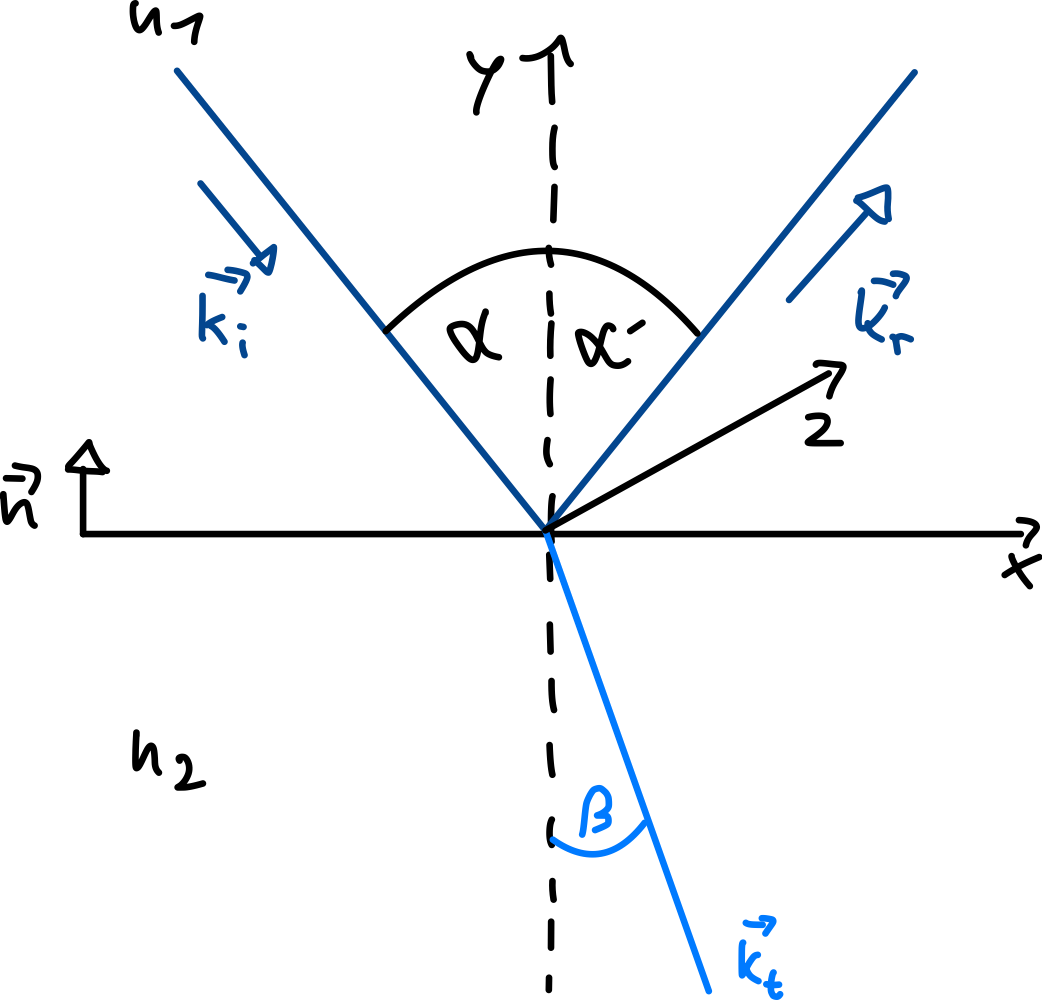
\includegraphics[width=0.25\textwidth]{Brechung.png}
%        \caption{asdf}
%\end{wrapfigure}
Lichtstrahl $\vv{k}_i$ trifft aus einem Medium $n_1$ in ein Medium $n_2>n_1$ und wird mit $\alpha $ zu $\vv{k}_r$ reflektiert. Das Licht wird auch um den Winkel $\beta $ (relativ zum Lot) gebrochen und verläuft mit $\vv{k}_t$ durch das Medium. Die $\vv{E}$--Felder sind dann
\begin{align} 
        \vv{E}_i&=\vv{E}_{0i}e^{\text{i}\left(\omega _it-\vv{k}_i\vv{r}\right)}\\
        \vv{E}_r&=\vv{E}_{0r}e^{\text{i}\left(\omega _rt-\vv{k}_r\vv{r}\right)}\\
        \vv{E}_t&=\vv{E}_{0t}e^{\text{i}\left(\omega _tt-\vv{k}_t\vv{r}\right)}
.\end{align} 
Das \textsc{Fermat}'sche Prinizp besagt, dass eine Welle immer den Weg der minimalsten optischen Laufzeit wählt. Es ist also möglich, dass sie in einem Medium mehr Zeit verbringt, bevor sie in das andere Medium wechselt.

\subsubsection{Stetigkeit}
Die Tangentialkomponente von $\vv{E}$ und $\vv{H}=\tfrac{1}{\mu \mu _0}\vv{B}$ sind an Grenzflächen stetig. Die Normalkomponente von $\vv{D}=\varepsilon \varepsilon _0\vv{E}$ und $\vv{B}$ sind an Grenzflächen stetig.\\\indent
Zunächst werden die $\vv{E}$--Felder betrachtet, wenn $\vv{r}=0$ ist.
\begin{align} 
        \vv{n}\times \left(\vv{E}_{0i}e^{\text{i}\omega _it}+\vv{E}_{0r}e^{\text{i}\omega _rt}\right)\stackrel{!}{=}\vv{n}\times \vv{E}_{0t}e^{\text{i}\omega _tt}
.\end{align} 
Diese Gleichung muss für beliebige Zeiten $t$ gelten. Es existiert nur eine nichttriviale Lösung wenn $\omega _r=\omega _i=\omega _t\equiv \omega $.
\\\hfill\\\textbf{Einschub}\\ 
An allgemeinen Grenzflächen bleibt die Frequenz gleich, also $\omega _{\,\text{vac}\,}=\omega _{\,\text{medium}\,}$,
\begin{align} 
        E=E_0\cos \left(kz-\omega t\right)=E_0\cos \left[k\left(z-\dfrac{\omega }{k}t\right)\right]
,\end{align} 
mit $\tfrac{\omega }{k}=\tfrac{c}{n}=v_{\,\text{ph}\,}$, also 
\begin{align} 
k_{\,\text{vac}\,}=\tfrac{k_{\,\text{medium}\,}}{n}\Leftrightarrow \dfrac{2\pi }{\lambda _{\,\text{vac}\,}}=\dfrac{2\pi }{\lambda _{\,\text{medium}\,}}\dfrac{1}{n}\Leftrightarrow \lambda _{\,\text{Medium}\,}=\dfrac{1}{n}\lambda _{\,\text{vac}\,}
.\end{align} 
Daraus folgt, dass $\omega =k\tfrac{c}{n}$.\\\indent
Jetzt ist $\vv{r}$ ein beliebiger Punkt auf der Grenzfläche, also
\begin{align} 
        \left.e^{\text{i}\omega t}\vv{n}\times \left(\vv{E}_{0,i}e^{-\text{i}\vv{k}_i\vv{r}}+\vv{E}_{r,0}e^{-\text{i}\vv{k}_r\vv{r}}-\vv{E}_{t,0}e^{-\text{i}\vv{k}_t\vv{r}}\right)\right|_{y=0}=0
.\end{align} 
Es muss für beliebiges $\vv{r}$ auf der Grenzfläche gelten
\begin{align} 
        \vv{k}_i\vv{r}=\vv{k}_r\vv{r}=\vv{k}_t\vv{r}\qquad \,\forall \vv{r}=\begin{pmatrix}
                x\\0\\z
        \end{pmatrix}
.\end{align} 
Für das einfallende Lichtfeld setzt man
\begin{align} 
        \vv{k}_i=\begin{pmatrix}
                k_{i,x}\\k_{i,r}\\0
        \end{pmatrix}
.\end{align} 
Daraus folgt
\begin{align} 
        \begin{pmatrix}
                k_{i,x}\\k_{i,r}\\0
        \end{pmatrix}\cdot \begin{pmatrix}
                x\\0\\z
        \end{pmatrix}=\begin{pmatrix}
                k_{r,x}\\k_{r,y}\\k_{r,z}
        \end{pmatrix}\begin{pmatrix}
                x\\0\\z
        \end{pmatrix}=\begin{pmatrix}
                k_{z,x}\\k_{t,y}\\k_{t,z}
        \end{pmatrix}\begin{pmatrix}
                x\\0\\z
        \end{pmatrix}
.\end{align} 
Das heißt, auch die reflektierten und transmutierten Strahlen bleiben in der Zeichenebene. Das gilt auch für
\begin{align} 
        k_{r,x}&=k_{i,x}&k_r\sin \alpha '&=k_i\sin \alpha \\
        k_{t,x}&=k_{i,x}&k_t\sin \beta &=k_i\sin \alpha 
.\end{align} 
Da $\omega $ immer gleich ist, ist $\tfrac{k}{n}$ konstant. Mit $k_i=k_r$ folgt $\alpha '=\alpha $. Aus den Gleichungen folgt auch, dass 
\begin{align} 
        k_t&=\dfrac{n_2}{n_1}k_i&n_1\sin \alpha &=n_2\sin \beta 
.\end{align} 
Diese Gleichung ist das \textsc{Snellius}'sche Brechungsgesetz. Für $n_2>n_1$ wird der Strahl zum Lot hin gebrochen.

\subsubsection{Die Amplitude von reflektiertem und gebrochenen Strahl}
Hier wird nur der Spezialfall des senkrecht Einfallenden Strahls betrachtet. Es gilt
\begin{align} 
        \vv{E}_{0,i}+\vv{E}_{0,r}&=\vv{E}_{0,t}\\
        n_1\left(\vv{E}_{0,i}-\vv{E}_{0,r}\right)&=n_1\vv{E}_{0,t}\\
        \vv{B}_{0,i}+\vv{B}_{0,r}&=\vv{B}_{0,t}
.\end{align} 
Der Zusammenhang zwischen den Feldern ist
\begin{align} 
        \vv{B}&=\dfrac{1}{\omega }\left(\vv{k}\times \vv{E}\right)&\vv{k}_r&=-\vv{k}_i
.\end{align} 
Aus diesen Gleichungen folgt
\begin{align} 
        E_{0,r}&=\dfrac{n_1-n_2}{n_1+n_2}\vv{E}_{0,i}&r&=\dfrac{n_1-n_2}{n_1+n_2}
,\end{align} 
mit $r$ dem Reflexionskoeffizienten. Für $n_2>n_1$, id est eine Relexion am optisch dichteren Medium, ist $r<0$, daraus folgt ein Phasensprung von $\pi $. Das $\vv{E}$--Feld dreht sich also um. Die reflektierte Intensität ist
\begin{align} 
        R&=\dfrac{I_r}{I_i}=|r|^2=\left(\dfrac{n_1-n_2}{n_1+n_2}\right)^2
.\end{align} 
All das was nicht reflektiert, wird transmutiert
\begin{align} 
        |r|^2+|t|^2&=R+T=1&t&=\dfrac{E_{0,t}}{E_{0,r}}
.\end{align} 
\hfill\\\textbf{Allgemeiner Fall}\\ 
Für das $\vv{E}_i$--Feld aus der Ebene der Brechung heraus und das $\vv{B}$--Feld orthogonal zu dem einfallenden Strahl in der Ebene gilt
\begin{align} 
        r_\perp &=\dfrac{-\sin \left(\alpha -\beta \right)}{\sin \left(\alpha +\beta \right)}&t_\perp&=\dfrac{2\sin \beta \cos \alpha }{\sin \left(\alpha +\beta \right)}
.\end{align} 
Für das $\vv{E}_i$--Feld orthogonal zu den einfallenden Strahlen in der Ebene gilt
\begin{align} 
        r_{| |}&=\dfrac{\tan \left(\alpha -\beta \right)}{\tan \left(\alpha +\beta \right)}&t_{| |}&=\dfrac{2\sin \beta \cos \alpha }{\sin \left(\alpha +\beta \right)\cos \left(\alpha -\beta \right)}
.\end{align} 

\subsubsection{\textsc{Brewster}--Winkel}
Der \textsc{Brewster}--Winkel ist der Winkel, bei dem polarisiertes Licht vollständig transmittiert und gar nicht reflektiert wird. Dieses Phänomen tritt auf, wenn reflektierter und gebrochener Strahl senkrecht aufeinander stehen ($r_{| |}=0$), also $\alpha +\beta =\ang{90}$. Der Winkel ist mit dem \textsc{Snellius}'schen Brechungsgesetz
\begin{align} 
        \tan \alpha _B&=\dfrac{n_2}{n_1}
.\end{align} 
Der Reflexionskoeffizient für einen streifenden Einfall geht gegen 1.

\subsubsection{Totalreflexion}
Licht wird von einem optisch dichteren in ein optisch dünneres Medium geschickt. Für $n_1\sin \alpha =n_2\sin \beta $ gibt es nur für den Fall $\sin \beta \leq 1$ und $\sin \alpha \leq \tfrac{n_2}{n_1}$ eine Lösung. Dies ist auch der Grenzwinkel für die totale Reflexion. Für $\alpha _g<\alpha $ wird alles Licht reflektiert.\\\indent
In Glasfaserkabeln wird sich die Totalreflexion zu nutze gemacht. Das Kabel ist ein Hohlzylinder, dessen Rand einen niedrigeren Brechungsindex $n_1<n_2$ hat, als der hohle Teil $n_2$ des Zylinders. Dadurch kann Licht über große Strecken versendet werden.\\\indent
Bei Totalreflelexion gibt es eine \textbf{evaneszent} abfallende Welle
\begin{align} 
        E\propto e^{-\tfrac{x}{\lambda }}
.\end{align} 
$k$ wird hier komplex.\\\indent
Für heiße Luftschichten ist der Brechungsindex proportional zu
\begin{align} 
        n\propto \dfrac{N}{V}=\dfrac{\rho }{k_BT}
.\end{align} 

\newpage
\section{Die elektromagnetische Welle in Materie}
\subsection{Absorption und Dispersion}
Als einfaches Modell wird angenommen, dass Materie aus vielen harmonischen Oszillatoren der Resonanzfrequenz $\omega _0$ besteht. Die Materie wird von einem elektrischen Feld durchsetzt
\begin{align} 
        E\left(t\right)&=E_0e^{-\text{i}\omega t}
.\end{align} 
Die Kraft, die auf das Elektron wirkt ist
\begin{align} 
        F\left(t\right)&=eE\left(t\right)=eE_0e^{-\text{i}\omega t}
.\end{align} 
Die Bewegungsgleichung ist
\begin{align} 
        \ddot{x}+\Gamma \dot{x}+\omega _0^2x=\dfrac{eE_0}{m}e^{-\text{i}\omega t}
.\end{align} 
Die Lösung dieser Gleichung funktioniert mit dem Ansatz $x\left(t\right)=x_0e^{-\text{i}\omega t}$. Die Amplitude ist
\begin{align} 
        x_0=\dfrac{eE_0}{m}\dfrac{1}{\omega _0^2-\omega ^2-\text{i}\Gamma \omega }
.\end{align} 
Ist die \textbf{Verstimmung} $\delta =\omega -\omega _0\ll \omega $, dann gilt
\begin{align} 
        \dfrac{1}{2\omega }\dfrac{1}{-\delta -\text{i}\tfrac{\Gamma }{2}}=\dfrac{1}{2\omega }\dfrac{-\delta +\text{i}\tfrac{\Gamma }{2}}{\delta ^2+\left(\tfrac{\Gamma }{2}\right)^2}
.\end{align} 
Die Materie ist ein \textbf{Polarisator} mit $P=Nex$ mit $N$ der Zahl der Oszillatoren pro Volumen. Die Suszeptibilität ist definiert als $\chi:=\tfrac{P}{\varepsilon _0E}$. Sie ist also komplex
\begin{align} 
        \chi=\dfrac{Ne^2}{\varepsilon _0m2\omega }\dfrac{-\delta +\text{i}\tfrac{\Gamma }{2}}{\delta ^2+\left(\tfrac{\Gamma }{2}\right)^2}
\end{align} 
\hfill\\\textbf{Veränderung des einfallenden Feldes}\\ 
Der komplexe Brechungsindex ist $\hat{n}=\mathcal{R}\left(\hat{n}\right)+\text{i}\mathcal{I}\left(\hat{n}\right)$.
\begin{align} 
        \dfrac{c}{\hat{n}}&=\dfrac{1}{\,\sqrt[]{\varepsilon _0\mu _0\varepsilon \mu }}
\end{align} 
Mit $\mu \approx 1$ ist $\hat{n}=\,\sqrt[]{\varepsilon }$. Die Polarisation ist also
\begin{align} 
        P&=\chi \varepsilon _0E\\
         &=\left(\varepsilon -1\right)\varepsilon _0E\\
         &=\left(\hat{n}-1\right)\varepsilon _0E
.\end{align} 
Die Suszeptibilität hat dann den Wert
\begin{align} 
        \chi=\left(\hat{n}^2-1\right)=\left(\hat{n}-1\right)\left(\hat{n}+1\right)\approx 2\left(\hat{n}-1\right)
.\end{align} 
Die Porportionalität des $\vv{E}$--Feldes ist
\begin{align} 
        E\propto e^{\text{i}\left(\omega t-kz\right)}&=e^{-\text{i}\omega \left(t-\hat{n}\tfrac{z}{c}\right)}\\
                                                     &=\underbrace{e^{-\mathcal{I}\left(\hat{n}\right)\omega \tfrac{z}{c} }}_{e^{-\tfrac{\alpha }{2}z}}e^{-\text{i}\omega \left(t-n \tfrac{z}{c}\right)}
\end{align} 
$\alpha $ ist der \textbf{Absorptionskoeffizient}. Die Proportionalitäten sind $I\propto |E|^2\propto e^{-\alpha z}$; $I=I_0e^{-\alpha z}$. $\alpha $ kann auch über den \textbf{Absorptionsquerschnitt} $\sigma $ berechnet werden, mit $\alpha =N\sigma $.\par
Für den Anteil von $\chi$ in Phase ist der Brechungsindex $n=1+\tfrac{1}{2}\mathcal{R}\left(\chi\right)$. Für den Anteil von $\chi$ $\ang{90}$ außer Phase ist $\alpha =\tfrac{\omega }{c}\mathcal{I}\left(\chi\right)$. Daraus folgt
\begin{align} 
        \,\text{Absorption}\,&:\alpha \left(\omega \right)=\dfrac{Ne^2}{2m\varepsilon _0c}\dfrac{\tfrac{\Gamma }{2}}{\delta ^2+\left(\tfrac{\Gamma }{2}\right)^2}\\
        \,\text{Dispersion}\,&:n=1+\dfrac{Ne^2}{4m\varepsilon _0\omega }\dfrac{-\delta }{\delta ^2+\left(\tfrac{\Gamma }{2}\right)^2}
.\end{align} 
Die Absorptionsresonanzen in der UV Wellenlänge bestimmen den Brechungsindex im sichtbaren Bereich. Hier ist bei der normalen Dispersion $\diff[]{n}{\omega }>0$ entsprechend $\diff[]{n}{\lambda }<0$.\par
Die Dispersion ist spektral breiter als die Absorption. Weit weg von der Resonanz ist sie proportional $\tfrac{1}{\omega -\omega _0}$ anstatt $\tfrac{1}{\left(\omega -\omega _0\right)^2}$ (wie bei der Absorption).

\subsubsection{Monochromatische Wellen}
Das Feld von monochromatischen Wellen ist
\begin{align} 
        E=E_0\cos \left[k\left(x-v_{ph}t\right)\right]
,\end{align} 
mit $v_{ph}=\tfrac{c}{n}$. Für die Ausbreitung von Wellenpaketen ist die Phasen und Gruppengeschwigkeit relevant.\par
Das Feld entlang der $z$--Achse ist 
\begin{align} 
        E\left(z,t\right)&=\dfrac{1}{2\pi }\int_{-\infty}^{\infty}E\left(\omega \right)e^{\text{i}\left(k\left(\omega \right)z-\omega t\right)}\td \omega 
,\end{align} 
mit $k\left(\omega \right)=\tfrac{\omega }{c}n\left(\omega \right)$ und $n\left(\omega \right)=n\left(\omega _{\,\text{max}\,}\right)+\diff[]{n}{\omega }\left(\omega -\omega _{\,\text{max}\,}\right)$.\par
Die Einhüllende des Pulses (id est das Maximum von $|E\left(z,t\right)|^2$) breitet sich mit $v_g=\diff[]{\omega }{k}$, $k=\tfrac{\omega }{c}n$, aus. Führt man diese Rechnung aus, gilt
\begin{align} 
        v_g=\dfrac{c}{n+\omega \diff[]{n}{\omega }}
.\end{align} 
Die Phasengeschwindigkeit ist $v_{ph}$, oberhalb der Resonanz $>c$. Die Gruppengeschwindigkeit ist $v_g=\diff[]{\omega }{k}<c$ (außer in Bereichen starker Absorption).

\subsection{Elektromagnetische Wellen in leitenden Medien}
Das Modell für diesen Fall ist ein freies Elektronengas. Das Feld des Lichts ist $E=E_0e^{\text{i}\omega t}$. Im bisherigen Modell geht $\omega _0$ gegen 0, da es keine Rückstellkraft gibt. Für hohe Frequenzen ist $\omega \gg \left(\,\text{Stoßzeit}\,\right)^{-1}$. Die Dämpfung $\Gamma $ wird auch 0. Die Bewegungsgleichung reduziert sich dann zu
\begin{align} 
        \ddot{x}&=\dfrac{eE\left(t\right)}{m}&\chi&=\dfrac{P}{\varepsilon _0E}=\dfrac{Nex}{\varepsilon _0E}=\dfrac{Ne^2}{\varepsilon _0m}\dfrac{1}{-\omega ^2}
,\end{align} 
mit $\varepsilon \left(\omega \right)=1+\chi=1-\tfrac{\omega _p^2}{\omega ^2}$ und $\omega _p^2=\tfrac{Ne^2}{\varepsilon _0m}$ als die Frequenz mit der das Plasma schwingt. Der Brechungsindex ist $n=\,\sqrt[]{\varepsilon }$. Unter der Plasmafrequenz absorbiert das leitende Material (z.B.\ Metall), über der Plasmafrequenz wird Metall durchsichtig.\par
Für das Feld im Medium und $\omega \ll \omega _p$ ist die Porportionalität 
\begin{align} 
        E\propto e^{- \mathcal{I}\left(\hat{n}\right)\omega z/c}=e^{-\mathcal{I}\left(\hat{n}\right)2\pi 2/\lambda }\qquad I\propto |E|^2\propto e^{-\mathcal{I}\left(\hat{n}\right)4\pi z\lambda }
.\end{align} 

\subsubsection{Reflexion an absorbierenden Medien}
Für den senkrechten Einfall ist 
\begin{align} 
        \hat{n}=\mathcal{R}\left(\hat{n}\right)+\text{i}\mathcal{I}\left(\hat{n}\right)
.\end{align} 
Der Reflexionsindex ist dann
\begin{align} 
        r=\dfrac{\hat{n}-1}{\hat{n}+1}\qquad R=|r|^2=\dfrac{\left(n-1\right)^2+\mathcal{I}^2\left(\hat{n}\right)}{\left(n+1\right)^2+\mathcal{I}^2\left(\hat{n}\right)}
.\end{align} 
Bei starker Absorption, also $\mathcal{I}\left(\hat{n}\right)\gg 1$ (ideal leitendes Metall für $\omega \ll \omega _p$), kommt es zu hoher Reflexion. Für Metalle besonders im Infrarotbereich. Im sichtbaren Sprektrum ist die Reflexion kleiner. Das Modell des Elektronengases ist schlechter für $\omega \approx \omega _p$.

\subsubsection{Farbe von Gegenständen}
Metalle besitzen eine hohe Leitfähigkeit. Dies führt zu einer breitbandigen hohen Reflexion und dem charakteristischen metallischen Glanz. Für Gold oder Kupfer (oder weitere) variiert die Relfexion in abhängigkeit von der Wellenläng ($R=R\left(\lambda \right)$). Dies führt zu einer Färbung.\par
Wenn bei Isolatoren keine Absorptionslinien im sichtbaren Spektralbereich vorhanden sind ist das Medium glasklar.\par
Inhomogene Oberflächen (z.B.\ Puder, raue Oberflächen) erscheinen weiß. Wasser ist fast glasklar, wohingegen Wasserdampf weiß erscheint.\par
Isolatoren mit schwacher Absorption haben die Farbe des transmutierten bzw.\ reflektierten Lichts. Isolatoren mit hoher Absorption haben einen metallischen Glanz.\\\indent
Gelbes Glas erschient geld, da blaues Licht absorbiert und nur rotes und grünes Licht reflektiert bzw.\ transmutiert wird. Die Mischung aus rot und grün ist gelb. Weitere Farben sind
\begin{align} 
        \,\text{magenta}\,&=\,\text{rot}\,+\,\text{blau}\,\\
        \,\text{cyan}\,&=\,\text{blau}\,+\,\text{grün}\,\\
        \,\text{gelb}\,&=\,\text{rot}\,+\,\text{grün}\,
.\end{align} 
Farbe kann auch durch Interferenz erzeugt werden.

\subsection{Streuung elektromagnetischer Wellen}
Weisses Licht wird an Molekülen in alle Richtungen gestreut. Wenn der Durchmesser der Moleküle $d$ viel kleiner als die Wellenlänge $\lambda $ ist, kommt es zur \textsc{Rayleigh}--Streuung. Die Streuung ist isotrop mit einem Wirkungsquerschnitt von
\begin{align} 
        \sigma =\dfrac{8\pi }{3}\left(\dfrac{e^2}{4\pi \varepsilon _0m_ec^2}\right)^2\dfrac{\omega ^4}{\left(\omega _0^2-\omega ^2\right)^2}
.\end{align} 
Für $\omega \ll \omega _0$ ist $\sigma \propto \omega ^4$, das heißt, blaues Licht wird stärker als rotes Licht gestreut. (Der Himmel ist blau, weil blaues Licht von den Molekülen der Atmosphäre gestreut wird. Abends erscheint der Himmel rot, da das Licht eine größere Strecke durch die Atmosphäre zurücklegt und mehr rotes transmutiertes Licht ankommt.)\par
Für $\omega \approx \omega _0$ kommt es zu einer Resonanzstreuung. Für $\omega \gg \omega _0$, sowie die Streuung an freien Elektronen (und keine Rückstellkräfte, also $\omega _0\rightarrow 0$), kommt es zur \textsc{Thomson}--Streuung, mit einem Wirkungsquerschnitt von
\begin{align} 
        \sigma =\dfrac{8\pi }{3}\left(\dfrac{e^2}{4\pi \varepsilon _0m_ec^2}\right)^2
.\end{align} 
Sie ist unabhängig von der Lichtwellenlänge.

\newpage
\section{Geometrische Optik}
Die Konzepte in diesem Kapitel sind allgemein gültig, wenn alle Dimensionen viel größer als die Wellenlänge sind.\\\indent
Die ebene Welle bleibt weiterhin $E=E_0\cos \left(kz-\omega t\right)$. Die Beugungseffekte am Rand von Lichtbündeln werden vernachlässigt.\\\indent
Die Grundaxiome der geometrischen Optik sind:
\begin{enumerate}[label=\roman*)]
        \item In einem optisch homogenen Medium laufen die Lichtstrahlen geradlinig.
        \item An Grenzflächen zwischen zwei Medien wird Licht gemäß des \textsc{Snellius}'schen Brechungsgesetzes reflektiert.
        \item Strahlen, die sich durchdringen, beeinflussen sich im Rahmen der linearen Optik nicht.
\end{enumerate}
Die allgemeine Formulierung der ersten zwei Punkte ist das \textsc{Fermat}'sche Prinzip der minimalen optischen Laufzeit zwischen zwei Punkten $P_1$ und $P_2$. Die Variation des Weges über die räumlich inhomogene Brechzahl muss also verschwinden,
\begin{align} 
        \delta \int\limits_{S\left(P_1\rightarrow P_2\right)}^{}n\left(\vv{r}\right)\td s=0
.\end{align} 
Die Interpretation davon ist, dass alle Wege außer des extremalen Wegs gemittelt werden und nur der extremale übrig bleibt.

\subsection{Optische Abbildung}
Die Motivation der optischen Abbildung ist das Sammeln von z.B.\ einer Lampe ausgesendeten Lichtstrahlen.
\\\hfill\\\textbf{Reelle Abbildung}\\ 
Ein Objekt (z.B.\ eine Lampe) kann mit Hilfe eines abbildenden Instruments (z.B.\ einer Linse) auf einem Schrim als ein reelles Bild abgebildet werden.
\\\hfill\\\textbf{Elliptische Spiegel}\\ 
Bei elliptischen Spiegeln werden alle Lichstrahlen, die von einem Brennpunkt ausgesendet werden, in den anderen Brennpunkt abgebildet.

\subsection{Sphärische Hohlspiegel / Kugelspiegel}
Sei ein Gegenstand auf der optischen Achse eines Hohlspiegels. Ein Lichtstrahl wird im Winkel $\gamma $ ausgesendet und um den Winkel $2\cdot \theta $ reflektiert. Der Mittelpunkt liegt auf der optischen Achse und wird um den Winkel $\theta $ refelktiert und kommt im Winkel $\alpha $ an. Der Bildpunkt befindet sich auf der optischen Achse und das Licht kommt im Winkel $\beta $ an.\\\indent
Der Abstand des Bildpunktes, des Mittelpunktes bzw.\ des Gegenstands zum Schnittpunkt von optischer Achse und Hohlspiegel ist $b,R$ bzw.\ $g$.\par
Ziel ist es, die Position des Bildpunktes als Funktion der Gegenstandsweite zu bestimmen. Mit dem Reflexionsgesetz gilt $\theta =\alpha -\gamma =\beta -\alpha \Leftrightarrow \beta +\gamma =2\alpha $. Hier kann die \textbf{paraxiale Näherung} verwendet werden. Diese Näherung besagt, dass alle Winkel sehr viel kleiner als 1 sind (achsnahe Strahlen). Zudem ist der Abstand $d$ zwischen dem Lot auf die optische Achse des Reflexionspunktes und dem Spiegel viel kleiner als alle anderen Längen. $h$ ist die Länge des Lots.\par
Die Näherungen sind dann 
\begin{align} 
        \tan \gamma &\approx \gamma \approx \dfrac{h}{g}\\
        \tan \alpha &\approx \alpha \approx \dfrac{h}{R}\\
        \tan \beta &\approx \beta \approx \dfrac{h}{b}
.\end{align} 
Aus $\beta +\gamma =2\alpha $ folgt dann
\begin{align} 
        \dfrac{1}{g}+\dfrac{1}{b}=\dfrac{2}{R}
.\end{align} 
Die Brennweite des Hohlspiegels ist definiert als
\begin{align} 
        f:=\dfrac{R}{2}
.\end{align} 
Für konvexe Spiegel ist $R<0$, also auch $f<0$.\par
Damit lässt sich das \textbf{Abbildungsgesetz} schreiben als
\begin{align} 
        \dfrac{1}{g}+\dfrac{1}{b}=\dfrac{1}{f}
.\end{align} 
Für $g\rightarrow \infty$ ist $b=f$.\par
Achsferne Strahlen, die in einem Winkel von z.B.\ $\ang{45}$ (zum Mittelpunkt) ankommen, werden wieder um $\ang{45}$ reflektiert. Die achsfernen Strahlen treffen sich mit den achsnahen Strahlen in einem Punkt. Die Abbildung ist nicht mehr scharf. Dieser Bildfehler lässt sich durch Verwendung eines Parabolspiegels vermeiden. Er lässt sich allerdings nur für die Fokussierung von parallelen Strahlen verwenden.

\subsection{Linsen}
Zunächst wird eine Abbildung durch eine brechende Kugelfläche betrachtet. Ein Lichtstrahl wird um den Winkel $\gamma $ zur optischen Achse ausgesendet und kommt in Einfallswinkel $\theta _1$ zur Normalen an. Der Lichtstrahl wird zum Lot hin um $\theta _2$ gebrochen. Der Abstand von Gegenstand zur Linse ist $g$; der Abstand von Bild zur Linse ist $b$. Der Abstand des Mittelpunktes $M$ zur Linse (die Weiterfühung der Normalen) auf der optischen Achse ist $R$. Der Einfallswinkel zum Bild ist $\beta $; der Einfallswinkel zum Mittelpunkt ist $\alpha $. Die Höhe des Reflexionspunktes über der optischen Achse ist $h$.\par
Das Brechungsgesetz ist dann $n_1\sin \theta _1=n_2\sin \theta _2$. In paraxialer Näherung gilt $n_1\theta _1=n_2\theta _2$. Zudem gilt $\theta _1=\gamma +\alpha $ sowie $\theta _2=\alpha -\beta $. Mit den Winkeln wie beim Hohlspiegel definiert ist das Gesetz
\begin{align} 
        n_1\left(\gamma +\alpha \right)&=n_2\left(\alpha -\beta \right)\\
        n_1\left(\dfrac{h}{g}+\dfrac{h}{R}\right)&=n_2\left(\dfrac{h}{R}-\dfrac{h}{b}\right)\\
        \dfrac{n_1}{g}+\dfrac{n_2}{b}&=\dfrac{n_2-n_1}{R}
.\end{align} 
Für eine dünne, auf beiden Seiten konvexe Linse, gilt für die Brechung an der Vorderseite bzw.\ an der Rückseite
\begin{align} 
        \dfrac{n_a}{g}+\dfrac{n_l}{b_1}&=\dfrac{n_l-n_a}{R_1}&\dfrac{n_l}{g_2(=-b_1)}+\dfrac{n_a}{b}&=\dfrac{n_a-n_2}{R_2}
.\end{align} 
Hier ist $n_l$ der Brechungsindex in der Linse und $n_a$ der Brechungsindex außerhalb der Linse. Alle 1--er Indizes sind vor der Linse, alle 2--er Indizes sind hinter der Linse.\par
Für $n_a=1$ (also Luft), und $n_l=n$, gilt für die Brennweite einer dünnen Linse
\begin{align} 
        \dfrac{1}{f}&=\left(n-1\right)\left(\dfrac{1}{R_1}-\dfrac{1}{R_2}\right)
.\end{align}
Das Inverse der Brennweite wird auch als \textbf{Brechkraft} $D:=\tfrac{1}{f}[\,\text{Dioptrie}\,]$ definiert.

\subsubsection{Virtuelle Abbilldungen}
Abbildende Instrumente beeinflussen die Lichtstrahlen so, das sie dem Beobachter vom Ort des Bildes herkommenden erscheinen.
Virtuelle Bilder können nicht mit einem Schrim aufgefangen werden (sie müssten mit einer weiteren Linse scharf gestellt werden).\par

\subsubsection{Abbildungen mit Linsen}
Für die allgemeine Konstruktion eines Bildes sind zwei Strahlen ausreichend. Es gibt verschiedene ausgezeichnete Strahlen die wie folgt konstruiert werden können.
\begin{enumerate}[label=\roman*)]
        \item Der Strahl parallel zur optischen Achse. Dieser geht durch den bildseitigen Brennpunkt.
        \item Der Strahl durch den Mittelpunkt der Linse. Dieser wird nicht abgelenkt.
        \item Der Strahl durch den gegenstandsseitigen Brennpunkt. Dieser verläuft hinter der Linse parallel zur optischen Achse.
\end{enumerate}
Man definiert die transversale Vergrößerung
\begin{align} 
        V_T&=\dfrac{B}{G}=\dfrac{f}{f-g}
.\end{align} 
Für $g>f$ ist $V_T<0$, das Bild steht also auf dem Kopf. $|V_T|$ wächst, wenn $g$ sich dem Brennpunkt nähert.

\subsubsection{Dicke Linsen}
Wenn die Dicke der Linse gegenüber $g,f,R_1$ und $R_2$ nicht mehr vernachlässigbar ist.\par
Um das übliche Verfahren zur Bildkonstruktion zu verwenden, wird das Licht nicht mehr an den Oberflächen der Linse gebrochen, sondern an zwei Hauptebenen im Abstand $h_1$ und $h_2$ von der Mitte der Linse.
Zwischen den Hauptebenen verlaufen die Strahlen parallel.
Es gilt
\begin{align} 
        h_{1,2}&=\dfrac{\left(n-1\right)fd}{nR_{1,2}}&\dfrac{1}{f}&=\left(n-1\right)\left[\dfrac{1}{R_1}-\dfrac{1}{R_2}+\dfrac{\left(n-1\right)d}{nR_1R_2}\right]
.\end{align} 

\subsection{Vergrößernde optische Instrumente}
Man definiert die \textbf{Vergrößerung} (oder auch \textbf{Winkelvergrößerung}) als
\begin{align} 
        V&:=\dfrac{\text{Sehwinkel mit Instrument}}{\text{Sehwinkel ohne Instrument}}=:\dfrac{\varepsilon _1}{\varepsilon _0}
.\end{align} 
Der Sehwinkel ohne Instrument ist auch der Sehwinkel im Abstand von dem kleinsten Abstand $S_0$, bei dem der Gegenstand noch scharf abgebildet werden kann.\par
Eine Lupe ist eine Sammellinse mit kurzer Brennweite und $g<f$. Die Vergrößerungen lassen sich ohne Lupe mit $\varepsilon _0=\tfrac{G}{S_0}$ und mit Lupe $\varepsilon =\tfrac{G}{g}\approx \tfrac{G}{f}$. Damit ist die Vergrößerung
\begin{align} 
        V=\dfrac{S_0}{f}
.\end{align} 

\newpage
\section{Matrizenoptik}
Das Ziel in der Matrizenoptik ist die Berechnung von optischen Systemen mit mehreren Linsen.
Für achsnahe Strahlen ist auch hier eine Linearisierung möglich. 
Mit paraxialer Optik sind für die Ausbreitung entlang einer Achse alle Winkel viel kleiner als 1.\par
Die Beschreibung der Strahlen erfolgt durch den Strahlvektor
\begin{align} 
        \vv{r}\left(z\right)&=\begin{pmatrix}
                r\left(z\right)\\\alpha \left(z\right)
        \end{pmatrix}
,\end{align} 
mit $r\left(z\right)$ dem Abstand und $\alpha \left(z\right)$ dem Winkel zur optischen Achse $z$.\par
Trifft ein Strahl $\vv{r}_1\left(z\right)$ in ein Medium und verlässt dieses wieder mit $\vv{r}_2\left(z\right)$, gilt 
\begin{align} 
        \vv{r}_2&=\hat{M}\vv{r}_1&\hat{M}&=\begin{pmatrix}
                A&B\\C&D
        \end{pmatrix}
.\end{align} 
Für ein paraxiales optisches System gilt
\begin{align} 
        \hat{M}_{\,\text{ges}\,}&=\hat{M}_i\cdot \hdots \cdot \hat{M}_2\cdot \hat{M}_1
.\end{align} 

\subsection{Beispiel: Ungestörte Fortpflanzung}
Für eine unegestörte Fortpflanzung (ohne Brechung) gilt $r_2=r_1+\alpha l$ und $\alpha _1=\alpha _2$, also
\begin{align} 
        \begin{pmatrix}
                r_2\\\alpha _2
        \end{pmatrix}&=\begin{pmatrix}
                r_1+\alpha _1l\\\alpha _1
        \end{pmatrix}\\
        &=\begin{pmatrix}
                1&l\\0&1
        \end{pmatrix}\begin{pmatrix}
                r_1\\\alpha _1
        \end{pmatrix}
.\end{align} 
Es bestägigt also die Relation 
\begin{align} 
        \vv{r}_2&=\hat{M}\vv{r}_1&\hat{M}&=\begin{pmatrix}
                1&l\\0&1
        \end{pmatrix}
.\end{align} 

\subsection{Beispiel: Dünne Linse}
Für eine dünne Linse mit Brennweite $f$ gilt $r_1=r_2$ und $\alpha _2=\alpha _1\tfrac{r_1}{f}$, also
\begin{align} 
        \hat{M}&=\begin{pmatrix}
                1&0\\-\tfrac{1}{f}&0
        \end{pmatrix}
.\end{align} 

\subsection{Beispiel: Sphärischer Spiegel}
Für eine sphärischen Spiegel mit Krümmungsradius $R$ und Brennweite $f=\tfrac{R}{2}$ gilt
\begin{align} 
        \hat{M}&=\begin{pmatrix}
                1&0\\-\tfrac{2}{R}&1
        \end{pmatrix}
.\end{align} 

\subsection{Beispiel: Zwei Linsen hintereinander}
Mit der Matrixmethode kann unmittelbar die Wirkung von zwei Linsen hintereinander bestimmt werden.\par
Der Abstand der Linsen mit Brennweiten $f_1$ und $f_2$ sei $d$. Es ist
\begin{align} 
        \hat{M}_{\,\text{ges}\,}&=\hat{M}_2\cdot \hat{M}_d\cdot \hat{M}_1\\
                                &=\begin{pmatrix}
                                        1&0\\-\tfrac{1}{f_2}&1
                                \end{pmatrix}\cdot \begin{pmatrix}
                                        1&d\\0&1
                                \end{pmatrix}\cdot \begin{pmatrix}
                                        1&0\\-\tfrac{1}{f_1}&1
                                \end{pmatrix}\\
                                &=\begin{pmatrix}
                                        1-\tfrac{d}{f_1}&d\\
                                        -\left(\tfrac{1}{f_1}+\tfrac{1}{f_2}-\tfrac{d}{f_1f_2}\right)&1-\tfrac{d}{f_2}
                                \end{pmatrix}
.\end{align} 
Das System zeigt gewisse Analogien mit einer einzigen Linse der Brennweite $\tfrac{1}{f}=\tfrac{1}{f_1}+\tfrac{1}{f_2}-\tfrac{d}{f_1f_2}$.\par
Es gibt folgende interessante Grenzfälle
\begin{enumerate}[label=\roman*)]
        \item Abstand $d\rightarrow 0$: Das System verhält sich nun wie eine einzige Linse mit Brennweite $\tfrac{1}{f}=\tfrac{1}{f_1}+\tfrac{1}{f_2}$ oder $D=D_1+D_2$ und $\begin{pmatrix}
                        1&0\\-\tfrac{1}{f}&1
        \end{pmatrix}$.
        \item Abstand $d=f_1+f_2$: Die Matrix hat dann die Form $\begin{pmatrix}
                        1-\tfrac{f_1+f_2}{f_1}&f_1+f_2\\0&1-\tfrac{f_1+f_2}{f_2}
        \end{pmatrix}$. Sind die Strahlen anfänglich parallel, dann bleibt die Steigung vor und nach dem Linsensystem identisch; die Strahlen werden aufgeweitet oder zusammengezogen.
\end{enumerate}

\newpage
\section{Linsenfehler}
Bisher war immer die Annahme, dass Linsen ideale optische Abbildungen erstellt haben. Linsen haben allerdings Fehler.

\subsection{Chromatische Abberation}
Weiterhin ist die Brennweite
\begin{align} 
        D=\dfrac{1}{f}&=\left(n-1\right)\left(\dfrac{1}{R_1}-\dfrac{1}{R_2}\right)
.\end{align} 
Allerdings hängt der Brechungsindex $n=n\left(\lambda \right)$ von der Wellenlänge $\lambda $ ab.
Wenn also weißes Licht an einer Linse gebrochen wird, ist bei normaler Dispersion $f_{\text{blau}}<f_{\text{rot}}$. 
Die Bildweite von blauem Licht ist kleiner als die Bildweite von rotem Licht.
Die transversale Vergrößerung ist also abhängig von der Wellenlänge.
Aus unterschiedlichen Glassorten zusammengesetzten Linsen kann die chromatische Abberation reduziert werden.

\subsubsection{Beispiel: Zweilinsiger Achromat}
Bei einem zweilinsigen (oder auch mehrlinsigen) Achromat werden zwei Linsen hintereinander gestellt, um der chromatischen Abberation entgegenzuwirken.
Die Gesamte Brechkraft ist dann
\begin{align} 
        D&=D_1+D_2&D_i\left(\lambda \right)&=\left(n_i\left(\lambda \right)-1\right)\rho _i
,\end{align} 
mit $\rho _i:=\left(\tfrac{1}{R_{i,1}}-\tfrac{1}{R_{i,2}}\right)$.\par
Mit so einem Zweilinser kann erreicht werden, dass die Brennweite für zwei Wellenlängen gleich ist.
Üblich sind $\lambda _1=\SI{656}{nm}$ und $\lambda _2=\SI{486}{nm}$.
Es soll also gelten
\begin{align} 
        D\left(\lambda _1\right)&=D\left(\lambda _2\right)\\
        \left(n_1\left(\lambda _1\right)-1\right)\rho _1+\left(n_2\left(\lambda _1\right)-1\right)\rho _2&\stackrel{!}{=}\left(n_1\left(\lambda _2\right)-1\right)\rho _1+\left(n_2\left(\lambda _2\right)-1\right)\rho _2
.\end{align} 
Damit liegt $\rho _1/\rho _2$ fest.\par
Die Angabe der Brennweite erfolgt üblicherweise bei der Wellenlänge von $\lambda _\alpha =\SI{587}{nm}$.
Die Angabe der Dispersion erfolgt über die \textsc{Abbe}--Zahl $\nu =\tfrac{n\left(\SI{587}{nm}\right)-1}{n\left(\SI{486}{nm}\right)-n\left(\SI{656}{nm}\right)}$. 
Gläser hoher bzw.\ kleiner Dispersion sind Flint--Gläser bzw.\ Kron--Gläaser.
Es gilt dann
\begin{align} 
        \nu _1f_1+\nu _2 f_2=0
.\end{align} 

\subsubsection{Monochromatische Abberation}
Bei der monochromatischen Abberation treten durch Verwendung der Näherung $\sin \varphi \approx \varphi -\tfrac{\varphi ^3}{3!}$ Bildfehler dritter Ordnung auf.

\subsubsection{Sphärische Abberation}
Kügelförmig geschliffene Linsen zeigen für Randstrahlen andere Brennweiten als für achsnahe Strahlen. 
Dies gilt sowohl für dicke, als auch für dünne Linsen.

\subsection{Weitere Bildfehler}
\begin{enumerate}[label=\roman*)]
        \item Koma: Strahlen, die schräg durch eine Linse fallen, haben asymmetrische Fehler.
Die Strahlen die durch die Mitte der Linse gehen treffen sich also an einem anderen Ort, als die Strahlen, die durch den Rand der Linse gehen.
        \item Astigmatismus: Die Brennebene in der $x$--Richtung ist anders, als die Brennebene in $y$--Richtung.
Dies tritt zum Beispiel auf, wenn eine Linse schräg durchlaufen wird.\par
Zylinderlinsen weisen einen extrem starken Astigmatismus auf.
        \item Verzeichnung: Bei der Verzeichnung werden parallele Linien gekrümmt.
        \item Bildfeldwölbung: Bei der Bildwölbung ist nur die Bildmitte oder der Bildrand scharf.
\end{enumerate}
Abbildungsfehler speilen meist bei großen Aperturen eine Rolle.
Man verwendet eine Blende um die Strahlen außen möglichst zu verringern.\par
Man definiert die \textbf{Blendenzahl} $F$ eines Objektives als
\begin{align} 
        F:=\dfrac{f}{D}
.\end{align} 
Eine große Blendenzahl bedeutet, dass der Durchmesser der Blende kleiner wird.



%}}}

\end{document}
